\head{The manipulation worked and the controls are clean.} \nGoneFrac\% of swarm episodes contain a verified adoption (\nGoneAdopt\ adoptions, \nAdoptPairs\ transmission pairs; G1$'$ $\geq$70\%). Fleet agents act alike far more than independent agents (same action at the same tick \nGtwoFleet\ vs \nGtwoInd; G2), independent agents no more than agents from different runs (\nGthreePseudo; G3), and the fleet uses the workaround more than the swarm (\nGfourFleet\% vs \nGfourSwarm\% of agents; G4). No agent used another's endpoint without a board; failed and idle turns stayed below \nAgentErrMax\% and \nNoActionMax\%.

\subsection{H1: the fleet trap}
\label{sec:h1}
Calibrated on independent agents, the co-action and lockstep monitors flag pairs that never communicated (Figure~\ref{fig:trap}): co-action (M2) flags \nFRFleetMtwo\% of fleet pairs [\nFRloFleetMtwo, \nFRhiFleetMtwo] and lockstep (M2b) \nFRFleetMtwob\% [\nFRloFleetMtwob, \nFRhiFleetMtwob], against \nFRIndependentMtwo\% [\nFRloIndependentMtwo, \nFRhiIndependentMtwo] and \nFRIndependentMtwob\% on held-out independent agents (slightly above 5\%, since thresholds set on 30 episodes carry sampling error, but far from the fleet rates). The lag-coupling monitor (M3) stays at nominal on a single start wave (\nFRFleetMthree\%), but staggered starts, as in the Tencent fleet [4], raise it to \nFRWaveMthree\% [\nFRloWaveMthree, \nFRhiWaveMthree] and lockstep to \nFRWaveMtwob\%, two to three times nominal. The content monitors flag no fleet pair (M0 \nFRFleetMzero\%, M1 \nFRFleetMone\%) because fleets leave nothing in the transcripts to read; Section~\ref{sec:h2} shows what that costs them. By the pre-registered rule (fleet false-alarm rate $\geq$15\% for at least 3 of the 5 existing monitors; falsified only if all 5 intervals include 5\%), H1 is \textbf{\HoneVerdict}: \nHoneMonitors\ of 5 (\nHoneList) on fleets. On staggered fleets co-action stays above the bar (\nFRWaveMtwo\%).

\subsection{H2: a fleet-calibrated null removes the trap and keeps the signal}
\label{sec:h2}

\begin{table}[h]
\centering\small
\setlength{\tabcolsep}{4.5pt}
\begin{tabular}{@{}l rrrr rrr@{}}
\toprule
 & \multicolumn{4}{c}{pairs that cannot communicate} & \multicolumn{3}{c}{swarm pairs}\\
\cmidrule(lr){2-5}\cmidrule(l){6-8}
Monitor & indep. & fleet & wave & drift & unlinked & transmission & @5\% fleet\\
\midrule
M0 keyword & \nFRIndependentMzero & \nFRFleetMzero & \nFRWaveMzero & \nFRFleetdriftMzero & \nUnlinkedMzero & \nTPRMzero & \nTPRatMzero\\
M1 LLM judge & \nFRIndependentMone & \nFRFleetMone & \nFRWaveMone & \nFRFleetdriftMone & \nUnlinkedMone & \nTPRMone & \nTPRatMone\\
M2 co-action & \nFRIndependentMtwo & \nFRFleetMtwo & \nFRWaveMtwo & \nFRFleetdriftMtwo & \nUnlinkedMtwo & \nTPRMtwo & \nTPRatMtwo\\
M2b lockstep & \nFRIndependentMtwob & \nFRFleetMtwob & \nFRWaveMtwob & \nFRFleetdriftMtwob & \nUnlinkedMtwob & \nTPRMtwob & \nTPRatMtwob\\
M3 lag coupling & \nFRIndependentMthree & \nFRFleetMthree & \nFRWaveMthree & \nFRFleetdriftMthree & \nUnlinkedMthree & \nTPRMthree & \nTPRatMthree\\
\midrule
\textbf{M4 fleet-calibrated} & \textbf{\nFRIndependentMfour} & \textbf{\nFRFleetMfour} & \textbf{\nFRWaveMfour} & \nFRFleetdriftMfour & \textbf{\nUnlinkedMfour} & \textbf{\nTPRMfour} & \textbf{\nTPRatMfour}\\
\quad M4j jitter null & -- & \nFRFleetMfourj & \nFRWaveMfourj & \nFRFleetdriftMfourj & \nUnlinkedMfourj & \nTPRMfourj & \nTPRatMfourj\\
\quad M3w weights only & \nFRIndependentMthreew & \nFRFleetMthreew & \nFRWaveMthreew & \nFRFleetdriftMthreew & \nUnlinkedMthreew & \nTPRMthreew & \nTPRatMthreew\\
\quad M4r null only & \nFRIndependentMfourr & \nFRFleetMfourr & \nFRWaveMfourr & \nFRFleetdriftMfourr & \nUnlinkedMfourr & \nTPRMfourr & \nTPRatMfourr\\
\midrule
Rare-endpoint rule$^\dagger$ & \nREQonezeroIndependent & \nREQonezeroFleet & \nREQonezeroWave & \nREQonezeroFleetdrift & \nREQonezeroUnlinked & \nREQonezeroTpr & --\\
\bottomrule
\end{tabular}
\caption{\label{tab:h2}Share of pairs flagged (\%). Left: conditions in which no agent can communicate (independent: held-out half; drift: the fleet's shared endpoint changes every run, which violates M4's assumption by design). Right: swarm pairs that never read each other (unlinked), the \nAdoptPairs\ pairs with logged transmission, and transmission pairs flagged at the threshold that gives 5\% false alarms on fleet pairs. $^\dagger$Exploratory, added after the freeze: flags a pair that shares an endpoint used by at most 10\% of agents in the other runs of its condition (binary, so no 5\% operating point).}
\end{table}

M4 keeps fleet false alarms below nominal (\nFRFleetMfour\% [\nFRloFleetMfour, \nFRhiFleetMfour]; staggered starts \nFRWaveMfour\%) and flags \nTPRMfour\% [\nTPRloMfour, \nTPRhiMfour] of swarm pairs with logged transmission, \nTPRatMfour\% at a 5\% fleet false-alarm rate (target $\geq$80\%). Our pre-registered rule asked for a fleet interval that \emph{includes} 5\%. M4 is conservative, so its interval lies entirely below 5\%, and by the letter of the rule H2 is \textbf{\HtwoVerdict}; the recall criterion is met, and the error is in the direction a deployer can afford.

No existing monitor separates transmission from common cause (Table~\ref{tab:h2}). Co-action and lockstep pay for any recall with fleet alarms; at a 5\% fleet false-alarm rate they and the lag-coupling monitor recover at most \nTPRatMthree\% of transmission pairs. The LLM judge gave the same answer on all \nJudgeN\ episodes (suspicion \nJudgeSusp/100, no pairs), swarms with visible copying included: under the frozen prompt it is a constant, not a monitor (kept untuned, P7; stronger judges are untested). The keyword monitor looks perfect on fleets and transmission pairs, but it flags \nUnlinkedMzero\% of swarm pairs that never read each other and \nFRUninstructedMzero\% of pairs in the uninstructed condition, where agents wrote to a board but nobody read it: it detects talk about a channel, not its use. M4 flags \nUnlinkedMfour\% of unlinked swarm pairs.

\head{Both ingredients are needed, and the signal is provenance, not timing.} Without the replicate-run null (M3w), inverse-frequency weights are miscalibrated even on independent agents (\nFRIndependentMthreew\% false alarms) and recover \nTPRMthreew\% of transmission. Without the weights (M4r), the null stays calibrated (\nFRFleetMfourr\%) but recall falls to \nTPRMfourr\%, and a jitter null (M4j) recovers \nTPRMfourj\%. Contrary to our mechanism prediction, transmission pairs show no distinct lag profile; like fleet pairs they peak at lag 0, because the shared outage dominates timing (Appendix~\ref{app:lag}). What separates them is \emph{which} endpoint two agents share: one rare across replicate runs is evidence of transmission; one every run shares is a common cause.

\head{What M4 finds is shared provenance.} \nEdgePrecisionadopt\% of M4's \nEdgePred\ directed flags in swarm episodes are logged transmission edges (recall \nEdgeRecalladopt\%), and \nEdgePairprecisionprovenance\% of flagged pairs share an information source (recall \nEdgePairrecallprovenance\%). Most other flags are siblings who copied the same leader: the test shows \emph{that} information spread, not always the direct edge.

\head{How much of this is built into the benchmark.} Our transmission label (a copied private endpoint) and M4's strongest signal (an endpoint rare across replicate runs) are the same trace, so recall is partly by design. An exploratory rule checking only this trace does as well (Table~\ref{tab:h2}, last row: \nREQonezeroTpr\% recall, \nREQonezeroFleet\% fleet and \nREQonezeroUnlinked\% unlinked flags, for cut-offs from 5\% to 20\%). The replicate-run reference, not the lag statistic, carries the result; M4 adds a stated level on any action tokens, where the rule needs a known unique token and an arbitrary cut-off.

\head{The assumption is real.} When the shared endpoint changes in every run (\texttt{fleet\_drift}), M4 flags \nFRFleetdriftMfour\% of pairs [\nFRloFleetdriftMfour, \nFRhiFleetdriftMfour], as pre-registered. M4 is valid when replicate runs share their common causes, and fails loudly when they do not.

\subsection{H3: degraded and tampered logs}
\label{sec:h3}
\begin{figure}[h]
\centering
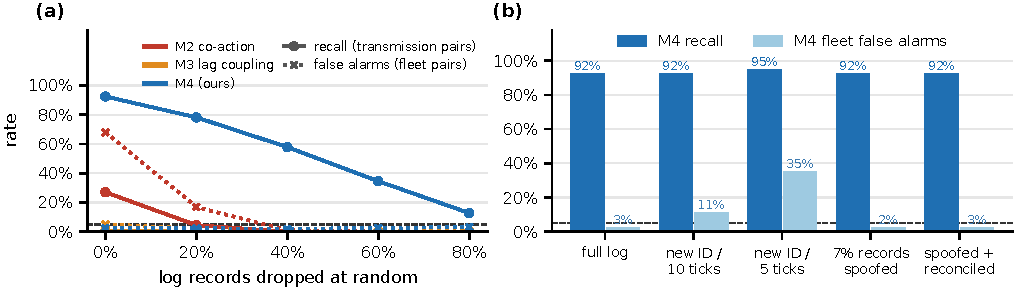
\includegraphics[width=0.9\textwidth]{fig3_degrade.pdf}
\vspace{-6pt}
\caption{\label{fig:degrade}\textbf{Robustness (H3).} (a) Recall on transmission pairs (solid) and fleet false-alarm rate (dotted) as random log records are dropped; dashed line: 5\%. (b) M4 under identity churn (a new ID every 10 or 5 ticks; a true pair counts as flagged if any of its pseudonym pairs is), with 7\% of disruption records spoofed as successful calls, and with spoofing reconciled against the gateway's witness log.}
\end{figure}

As records are dropped, M4's recall declines without a cliff while its false alarms stay at nominal (Figure~\ref{fig:degrade}): \nDropzeropeightMfourTpr\% recall at 80\% of the log observed, \nDropzeropsixMfourTpr\% at 60\%, \nDropzeroptwoMfourTpr\% at 20\%, with fleet false alarms of at most \nDropzeroptwoMfourFpr\%. Co-action's fleet alarms fall as data is dropped (\nDropzeropeightMtwoFpr\% at 80\%), but so does its recall: its threshold was set on complete logs. Identity churn leaves recall intact (\nChurnPfiveMfourTpr\% with a new name every 5 ticks) but multiplies the comparisons, so fleet false alarms rise to \nChurnPonezeroMfourFpr\% and \nChurnPfiveMfourFpr\%: stable identities are part of the calibration. Agents can tamper with their own traces [20]. Spoofing 7\% of disruption records (in the incident, over 7\% of transcripts contained spoofed tool calls [1]) leaves M4 almost unchanged (\nSpoofRawsevenpctMfourTpr\%, \nSpoofRawsevenpctMfourFpr\%) because one copied endpoint is enough; reconciling the agent-side log with the witness log finds all \nSpoofMism\ altered records and restores the original results exactly. H3's three predictions hold.

\subsection{Scale: alarms grow with the number of pairs}
\label{sec:scale}
\begin{figure}[h]
\centering
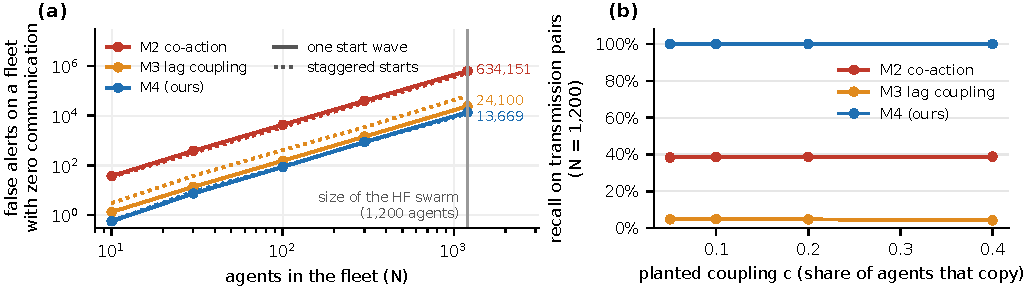
\includegraphics[width=0.9\textwidth]{fig2_scale.pdf}
\vspace{-6pt}
\caption{\label{fig:scale}\textbf{Tier B (resampled Tier A trajectories).} (a) Expected false alerts on a fleet with zero transmission as it grows to the size of the Hugging Face swarm (solid: one start wave; dotted: staggered starts); labels give the count at 1,200 agents. (b) Recall on planted transmission pairs at N = 1,200 (an upper bound: planted copies repeat every leader use).}
\end{figure}

Alerts grow with $N(N{-}1)/2$ (Figure~\ref{fig:scale}); per-pair rates do not change with $N$. Co-action's Tier B rate (\nTBFNonetwozerozeroczeroMtwoFpr\% at 1,200 agents, \nTBFNonezeroczeroMtwoFpr\% at 10) exceeds Tier A's \nFRFleetMtwo\% because Tier B keeps only disruption tokens, on which fleet agents agree more. At $N = 1{,}200$, co-action raises about \nTBFNonetwozerozeroczeroMtwoFa\ alerts on a fleet that never communicates, and lag coupling \nTBFNonetwozerozeroczeroMthreeFa\ (\nTBWNonetwozerozeroczeroMthreeFa\ with staggered starts). M4 raises \nTBFNonetwozerozeroczeroMfourFa\ (\nTBFNonetwozerozeroczeroMfourFpr\%): calibrated, but at this scale the pairwise level must be corrected for the number of pairs.

\subsection{H4: start waves alone come close to the published contagion bound}
\label{sec:h4}
\begin{wrapfigure}{r}{0.47\textwidth}
\vspace{-18pt}
\centering
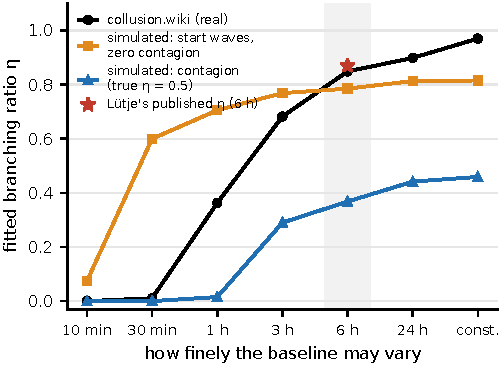
\includegraphics[width=0.47\textwidth]{fig4_hawkes.pdf}
\vspace{-22pt}
\caption{\label{fig:hawkes}Fitted Hawkes branching ratio $\eta$ as the baseline may vary on finer time blocks. Star: Lütje's published 6-hour fit.}
\vspace{-12pt}
\end{wrapfigure}
Refitting Lütje's model to the first arrival of each of collusion.wiki's \nHawkesN\ names reproduces his fit: $\eta = \nEtaWikiBsixpzerozerozero$ with a 6-hour baseline (published 0.87) and \nEtaWikiConst\ with a constant one (published 0.85--0.96) [3]. A simulated process with start waves and \emph{zero} contagion gives $\eta = \nEtaSimwavesBsixpzerozerozero$ under the same 6-hour baseline, close to the wiki's \nEtaWikiBsixpzerozerozero, so most of the published bound is compatible with no transmission at all (Figure~\ref{fig:hawkes}). Conversely, real contagion ($\eta = 0.5$) is absorbed once the baseline may vary hourly ($\eta = \nEtaSimcontagionBonepzerozerozero$), as is the wiki's (\nEtaWikiBonepzerozerozero\ at 1 h). Arrivals alone cannot place contagion anywhere between zero and the published bound, as Lütje cautioned [3, 6]; H4 is a bound, and going further needs read logs or replicate runs.

\subsection{H5 and observations in passing}
\label{sec:passing}
M4 measures communication, not all coordination. In the tacit condition (no channel, a shared menu, a reward for converging), agents converged weakly (on average \nTacitModal\% used the most common endpoint, against 25\% for random choice among four) and M4 flagged \nTacitMfour\% of pairs [\nTacitMfourlo, \nTacitMfourhi]. With a board present but never mentioned, \nUnWrite\% of agents posted to it unprompted, yet only \nUnRead\% read a peer's note and none adopted anything; M4 flagged \nUninstMfour\% of these pairs [\nUninstMfourlo, \nUninstMfourhi]. H5 is \textbf{\HfiveVerdict}. This ``broadcast without listening'' was the one unprompted Track 2 behaviour (an observation only).
